%% kut_econ_template_mac.tex
%%
%% 高知工科大学 経済・マネジメント学群 卒論テンプレート(macOS用)
%% R Markdown -> PDF 用
%%
%% Author: 矢内 勇生 (Yuki YANAI)  <yanai.yuki@kochi-tech.ac.jp>
%% Created: 2021-01-23
%% Modified:
%% 2021-11-27 YY: 二段組から一段組に変更, 表紙を追加
%% 2022-02-05 YY:
%%    kut_econ_thesis_lualatex.tex をベースに、OSごとにテンプレを分割。
%%    tabularx を追加。Rコードのshade を有効化。

\PassOptionsToPackage{unicode}{hyperref}
\PassOptionsToPackage{hyphens}{url}

\documentclass[lualatex,
               a4paper,
               10.5pt,
               ja=standard,
               jafont=ipaex]{bxjsarticle}
% フォントの設定: IPAex を採用
% 原ノ味フォントを使う場合 -> jafont=hiragino-pron を削除

\setpagelayout*{top=30truemm,bottom=30truemm,left=30truemm,right=30truemm}
\usepackage{amsmath,amssymb}
\usepackage{lmodern}
\usepackage{color}
\usepackage{natbib}
\bibpunct[:\,]{(}{)}{;}{}{}{,}
\usepackage{flafter}
\usepackage{tabularx}

\usepackage{luatexja}
\usepackage{luatexja-fontspec}

\usepackage{unicode-math}
\defaultfontfeatures{Scale=MatchLowercase}
\defaultfontfeatures[\rmfamily]{Ligatures=TeX,Scale=1}

\IfFileExists{upquote.sty}{\usepackage{upquote}}{}
\IfFileExists{microtype.sty}{
  \usepackage[]{microtype}
  \UseMicrotypeSet[protrusion]{basicmath}
}{}
\usepackage{xcolor}
\IfFileExists{xurl.sty}{\usepackage{xurl}}{}
\usepackage{bookmark,hyperref}
\hypersetup{
  pdftitle={研究内容が一目で分かるタイトルをつける},
  pdfauthor={宇畑優太},
  bookmarksnumbered=true,
  colorlinks=true,
  linkcolor=blue,
  urlcolor=cyan,
  citecolor=teal,
  hyperfootnotes=true,
  setpagesize=false,
  pdfcreator={LaTeX via pandoc from R Markdown}}
\urlstyle{same}
\usepackage{graphicx}
\makeatletter
\def\maxwidth{\ifdim\Gin@nat@width>\linewidth\linewidth\else\Gin@nat@width\fi}
\def\maxheight{\ifdim\Gin@nat@height>\textheight\textheight\else\Gin@nat@height\fi}
\makeatother
\setkeys{Gin}{width=\maxwidth,height=\maxheight,keepaspectratio}
\makeatletter
\def\fps@figure{htbp}
\makeatother
\setlength{\emergencystretch}{3em}
\providecommand{\tightlist}{%
  \setlength{\itemsep}{0pt}\setlength{\parskip}{0pt}}
\setcounter{secnumdepth}{5}
\usepackage{bookmark}
\usepackage{indentfirst}
\parindent=1em
\usepackage{dcolumn}
\newcolumntype{.}{D{.}{.}{-1}}
\usepackage{caption}
\captionsetup[table]{name=表}
\captionsetup[figure]{name=図}
\usepackage{selnolig}
\newlength{\cslhangindent}
\setlength{\cslhangindent}{1.5em}
\newlength{\csllabelwidth}
\setlength{\csllabelwidth}{3em}
\newenvironment{CSLReferences}[2] %
 {%
  \setlength{\parindent}{0pt}
  \ifodd #1 \everypar{\setlength{\hangindent}{\cslhangindent}}\ignorespaces\fi
  \ifnum #2 > 0
  \setlength{\parskip}{#2\baselineskip}
  \fi
 }%
 {}
\usepackage{calc}
\newcommand{\CSLBlock}[1]{#1\hfill\break}
\newcommand{\CSLLeftMargin}[1]{\parbox[t]{\csllabelwidth}{#1}}
\newcommand{\CSLRightInline}[1]{\parbox[t]{\linewidth - \csllabelwidth}{#1}\break}
\newcommand{\CSLIndent}[1]{\hspace{\cslhangindent}#1}

% Rコードを付録・補遺で表示する際に背景のshadeを有効に

  \title{\vspace{-28pt}{\Large\gtfamily\bfseries 研究内容が一目で分かるタイトルをつける}\thanks{ここに謝辞を書く。これは高知工科大学経済・マネジメント学群に提出する卒業論文を書くための R Markdown 用テンプレートである。草川孝夫先生の発案に基づき矢内勇生が作成した。デバッグに協力してくれた林良平氏とR Markdown で論文を書くことを可能にしてくれた Yihui Xie 氏に感謝する。このテンプレートに関する問い合わせは、矢内勇生 \textless{}\href{mailto:yanai.yuki@kochi-tech.ac.jp}{\nolinkurl{yanai.yuki@kochi-tech.ac.jp}}\textgreater{} まで。}}
  \usepackage{etoolbox}
  \makeatletter
  \providecommand{\subtitle}[1]{
    \apptocmd{\@title}{\par {\large #1 \par}}{}{}
  }
  \makeatother
  \subtitle{\large\gtfamily\bfseries \vskip 0.4em サブタイトルはあってもなくてもよい\vspace{-8pt}}
\author{\large 1260404 宇畑優太\\ 指導教員 矢内勇生}
\date{} % 日付は表示しない

% 節と小節のタイトルのフォントサイズを設定
%\usepackage{titlesec}
%\titleformat*{\section}{\large\selectfont\bfseries}
%\titleformat*{\subsection}{\normalsize\selectfont\bfseries}
%\titlespacing*{\section}{0pt}{2em}{4pt}
%\titlespacing*{\subsection}{0pt}{1.5em}{4pt}

\addtolength{\footskip}{10mm} % ページ番号を下にずらす
\renewcommand{\baselinestretch}{1.2} % 行間を調整
\renewcommand{\thefootnote}{\arabic{footnote}} % 脚注番号のラベルを変更


\begin{document}

%表紙
\thispagestyle{empty}
\begin{center}
\Large
高知工科大学 経済・マネジメント学群 \\
2021年度 卒業論文\\
\vspace{36truemm}
{\LARGE\gtfamily\bfseries 研究内容が一目で分かるタイトルをつける}\\
\vspace{4truemm}
  {\Large\gtfamily\bfseries サブタイトルはあってもなくてもよい}
\vfill
学籍番号 1260404 \\
\vspace{4truemm}
氏名 宇畑優太 \\
\vspace{8truemm}
指導教員氏名 矢内勇生
\end{center}

%要旨
\newpage
\maketitle
\thispagestyle{empty} %要旨が2頁以上になるときはコメントアウト
%\pagenumbering{roman} %要旨が2頁以上になるときはアンコメント

\noindent
\textbf{研究背景}

ここに研究の背景を書く。論文を書くたびにフォーマットに悩まされるのは時間の無駄だ。なんとか楽をしたい。

\vspace{4truemm}
\noindent
\textbf{研究目的}

ここに研究の目的を書く。R マークダウンファイルを knit して体裁の整ったPDFファイル生成することを目指す。

\vspace{4truemm}
\noindent
\textbf{研究方法}

ここに研究の方法を書く。knitr、pandoc、LuaLaTeX を利用する。

\vspace{4truemm}
\noindent
\textbf{分析結果}

ここに研究結果を書く。Rマークダウンファイルで卒論が書けるようになった。

\vspace{4truemm}
\noindent
\textbf{結論}

ここに研究の結果(と考察、インプリケーション)を書く。このテンプレートを利用すれば、Rマークダウンだけで卒業論文を書くことができる。Enjoy!

\newpage
\pagenumbering{arabic}

\section{序論(or はじめに)}\label{ux5e8fux8ad6or-ux306fux3058ux3081ux306b}

Rでデータを分析し、その結果を利用して卒業論文を執筆する学生には、このテンプレートで卒業論文を書くことを強く推奨する\footnote{Rでデータ分析を行わないとしても、\LaTeX よりもMarkdownのほうが使いやすいというなら、このテンプレートを使うのが簡単かもしれない。}。分析結果をアップデートする度に図表の挿入をやり直したり、本文中の数値を書き換えたりするのは大きな手間である。それはいかなる付加価値も生み出さない無駄な作業である。そして、そのような書き換え作業は思わぬミスを呼び込み、結果として再生不可能な結果を報告するという残念な帰結を生み出す。このテンプレートを使えば、分析と本文の作成に必要なすべてのコードを1つのファイルに記録することができる\footnote{矢内のやる気を喚起するという難しい仕事をやり遂げた草川先生に感謝したまえ。}。したがって、再生可能な研究の最低限の要件を満たすことが容易になるだろう\footnote{I will give you all my love. これまでの注の書き方をよく見ると、脚注の作り方が2通りあることがわかる。}。

このテンプレートは、フォントのサイズと種類の変更や、余白の設定、図表の挿入位置と通し番号の調整などの、研究とは無関係の難題から学生を解放する\footnote{R(と \LaTeX )の使い方を知っていると人生が楽になるという1つの例である。}。 論文を評価する際、研究の内容が最も重要な要素であることは言うまでもないが、形式の美しさを蔑ろにする論文には、研究の質の高さも期待できない\footnote{筆者はそのように信じている。しかし、この文のように根拠が明らかではない自分の思い込みを論文に書いてはいけない!論拠となる先行研究を明示するか、そのように考えられる理由を詳細かつ論理的に説明すること。}。

参考文献表の作成には BibTeX を利用する。参考文献は BibTeX 形式で \texttt{myrefs.bib} という名前のファイルに記録し、そのファイルを卒論のRmdファイルが保存されているディレクトリ(フォルダ)に保存する。BibTeX 自体の使い方を覚える必要はない\footnote{knit するときに自動的に実行される。}が、.bib ファイルの作り方は覚える必要がある\footnote{Zotero やJabRef、Mendeley などの文献管理アプリに書誌情報を入力し、BibTeX (.bib) 形式でエクスポートすればよい。}。詳しくは、皆さんの指導教員が教えてくれるだろう。

このテンプレート(Rmdファイル)をPDFに出力 (knit) すると、\texttt{kut\_econ\_thesis.pdf} ができる。正しく出力できれば、\texttt{kut\_econ\_thesis\_sample.pdf} と同じ見た目のファイルができるはずである。PDFの作成に使用する \LaTeX  のテンプレート (\texttt{kut\_econ\_template.tex}) も矢内が作った\footnote{よって、誤りが残されている可能性が高い。}。 LuaLaTeX の使用を想定しているので、LuaLaTeX が利用可能な TeX 環境がないと、このテンプレートは使えない。日本語フォントは、\href{https://moji.or.jp/ipafont/}{IPAexフォント} に設定してある\footnote{他のフォントを使いたい場合は \href{https://ja.osdn.net/projects/luatex-ja/wiki/LuaTeX-ja\%E3\%81\%AE\%E4\%BD\%BF\%E3\%81\%84\%E6\%96\%B9}{このウェブページ}を参考に、\LaTeX テンプレートを少し修正すればよい。IPAexフォントでも問題はないはずなので変える必要はないが、macOSではヒラギノフォントが使えるので、図のフォントとともにすべてヒラギノにしてもよい。2021年7月現在、日本語 \LaTeX  の標準フォントは\href{https://texwiki.texjp.org/?\%E5\%8E\%9F\%E3\%83\%8E\%E5\%91\%B3\%E3\%83\%95\%E3\%82\%A9\%E3\%83\%B3\%E3\%83\%88}{原ノ味フォント}であり、それを使ってもよい。ただし、そうするとRで作った図のフォントと本文のフォントが異なるものになってしまうので注意されたい。}。このフォントは標準ではインストールされていないかもしれない\footnote{macOSの場合、フォントブック (Font Book) というアプリでインストール済みのフォントが確認できる。Windows では、{[}コントロールパネル{]} -\textgreater{} {[}デスクトップのカスタマイズ{]} -\textgreater{} {[}フォント{]} でインストール済みのフォントが確認できる。Ubuntu では、ターミナルで \texttt{fc-list} を実行すればよい。IPAex を確認するだけなら、\texttt{fc-list\ \textbar{}\ grep\ ipaex} とすればよい。}。IPAexフォントがインストール済みでないなら、\href{https://moji.or.jp/ipafont/ipafontdownload/}{ダウンロードページ}で最新版を入手し、それをインストールしてほしい(明朝とゴシックの2書体が必要)。詳しくは、IPAexフォントの\href{https://moji.or.jp/ipafont/installation/}{インストール方法}を参照されたい。

このテンプレートを使って卒業論文を書く場合、\LaTeX  と BibTeX については、\citet{okumura2020} を軽く読めば(あるいは手元に置いて必要なときに参照すれば)万全である\footnote{この本は、このテンプレートを使おうと思う研究室には最低でも1冊ずつあるべき本なので、自分の研究室にない場合は指導教員に相談を。}。

\section{先行研究(この節タイトルはダサいので変える)}\label{ux5148ux884cux7814ux7a76ux3053ux306eux7bc0ux30bfux30a4ux30c8ux30ebux306fux30c0ux30b5ux3044ux306eux3067ux5909ux3048ux308b}

ここに先行研究のまとめを書く。ただし、節のタイトルは「先行研究」ではなく、先行研究が扱っているテーマがわかるように書く。

先行研究のまとめは、先行研究の単なる羅列や要約ではない。先行研究で何が明らかになり、何が明らかになっていないかを、論文ごとではなく、内容ごとにまとめる。同じ論点にかかわる先行研究が複数あれば、ひとつの段落で該当する複数の論文をまとめて整理する。論文1つにつき1つの段落を作れば良いというものではない。

論文は自分がどれだけ勉強したかを示す場ではないので、研究過程で読んだ本であっても、自らの論文の「論」に関係のない文献を取り上げてはいけない。自分の卒論と同じテーマを扱っているというだけでは、先行研究として取り上げるに値しない場合がほとんどである。先行研究の整理がきちんとできていれば、自分の研究とリサーチクエスチョンが同じか類似しているものだけが残されるはずである\footnote{自分のリサーチクエスチョンがどのような文脈に位置づけられるかを明らかにするために、広範囲にわたる先行研究を取り上げることもあり得る。しかし、できるだけ的を絞って先行研究をまとめたほうが良いだろう。}。

論文を読まなければ、論文は書けない。質の高い論文を読まなければ、質の高い論文は書けない。良い卒業論文を書きたいなら、質の高い論文をたくさん読むべし。

論文の質を判断するためには、ある程度の専門知識と経験が必要である。残念ながら、世の中には低品質の論文や本が多い。科学的根拠に乏しいデマや疑似科学にだまされることがないように、まずは各分野の教科書や評価の定まった古典的研究を読み、各分野の基礎を身に付けることが肝心である。どんな本や論文を読むべきかについては、各自の指導教員に相談すべきである。

何本の論文を先行研究として参照すべきかは扱う問題によって異なるので、参照すべき先行研究や論文・研究書の数を具体的な数値で提案することはできない。間違いなく言えることは、「良い論文を書きたいなら」それなり多くの論文を読まなければならないということである。自分の卒業論文で参照・引用する論文の数が15本だとしても、15本だけ読めば済むというものではない。

\section{理論と仮説}\label{ux7406ux8ad6ux3068ux4eeeux8aac}

自らの理論(卒業論文で主張する説)について、根拠を示しながら論理的に説明する。その理論をどうやって検証するかを明確にする。理論から観察可能な含意 (observable implications) を導き出し、観察可能な変数によって構成される作業仮説を提示する。

どのような証拠があれば仮説が支持されるかを明示するのは当然だが、どのような証拠があれば仮説が支持されないか(つまり、自分の説が誤りであることになるか)も明らかにすることが重要である。

\section{方法}\label{ux65b9ux6cd5}

\subsection{データ}\label{ux30c7ux30fcux30bf}

分析で使用するデータについて詳しく述べる。データをどこでどうやって手に入れたか(出所)、そのデータにどのような前処理を施したかを具体的に述べ\footnote{前処理については、Rmd ファイルにコードを書き、それを配布するのが理想である。}、論文の読者が完全に同じデータを手に入れることができるようにする。重要な変数の記述統計、ヒストグラム、散布図なども示すとよいだろう。

\subsection{分析手法}\label{ux5206ux6790ux624bux6cd5}

分析手法を明示する。統計分析をするなら、統計モデルを提示する。その際、分析上の仮定を明示するとともに、変数選択の根拠を示す必要がある。欠落変数バイアスや処置後変数バイアスが生じないと考えられる理論的根拠を説得的に示すことが求められる。

本文内数式は \(\bar{x} = \sum_{i=1}^n x_i / n\)のように書く。 \emph{This sentence is in italic}. ただし、日本語はイタリックにしない。 \textbf{太字}も書けるが論文では使わない。

独立行での数式は次のように書く。
\[
\bar{x} = \frac{1}{n} \sum_{i=1}^n x_i
\]

数式番号を付けたいときは \LaTeX  の\texttt{align}環境を使って次のように書く。
\begin{align}
f(x ; \mu, \sigma) = \frac{1}{\sqrt{2\pi \sigma^2}}
  \exp \left( -\frac{(x - \mu)^2}{2 \sigma^2} \right)
  \label{eqn:normal}
\end{align}

\texttt{\textbackslash{}label\{ラベル\}} でラベルを付けておけば、\texttt{\textbackslash{}ref\{ラベル\}} を使い、本文中で「式 (\ref{eqn:normal}) は正規分布の確率密度関数である」のように数式番号にアクセスできる。番号を自分で直接書かないので、他の式を挿入したり数式を提示する順番を変えたりして数式番号が変わっても、本文を書き換える必要はない。

複数行にわたる数式ブロックを書くときは、\texttt{aligned}環境(\texttt{align} ではない)を使い、\texttt{\&} で左右の位置を揃える。
\[
\begin{aligned}
  p(z | n, \theta) &= \binom{n}{z} \theta^{z} (1 - \theta)^{n - z}\\
  \binom{n}{z} &= {}_n C_z = \frac{n!}{z! (n - z)!}
\end{aligned}
\]
\noindent この文のように、数式ブロックの後に\textbf{段落を変えずに}文章を続けるときは \texttt{\textbackslash{}noindent} を忘れずに書く。

複数行で数式番号をつけるときは、\texttt{align}環境(\texttt{aligned} ではない)を使い次のようにする。
\begin{align}
  Y_i &\sim \mbox{Bernoulli}(\theta_i)  \label{eqn:likelihood} \\
  \log \left( \frac{\theta_i}{1 - \theta_i} \right) &=  \beta_0 + \beta_1 X_{i} + \beta_2 Z_{i} \label{eqn:link}
\end{align}
式 (\ref{eqn:likelihood}) と (\ref{eqn:link}) はそれぞれ尤度とリンク関数である。このように、\texttt{\$\$}を使わずに数式を書くときは、直後に文を続ければ \texttt{\textbackslash{}noindent}なしでも前の文と同じ段落として扱われる。段落を変えたいときは、通常の段落作成と同じように空行を入れれば良い。

\section{結果}\label{ux7d50ux679c}

分析結果は図や表で示すことが多いだろう。図や表にはそれぞれ別系統の通し番号を付ける必要があるが、それぞれの図表に他と重複のないラベルをつけておくと、番号は自動的に付される。したがって、適切なラベルさえ付けておけば、図や表を追加したり、図表の順番を入れ替えたりしても、手動で番号を付け直す必要はない。ラベルの付け方が特殊\footnote{\LaTeX  とよく似た方法ではあるが、まったく同じではないので注意が必要。}なので、しっかり身につけよう。

まず、表のラベルの付け方を説明する。表\ref{tab:reg1}は、気圧 (mm) を気温(摂氏)に回帰した線形回帰モデルのパラメタを推定した結果である。モデル (1) は単回帰、モデル (2) は気温の2乗を説明変数に加えた重回帰である。現代の標準的作法に従えば、回帰分析の結果は表ではなく図で示すべきだが、表の作り方を説明するためにあえて表を示す。

\begin{table}[t]
\caption{推定結果:応答変数は気圧 (mm)}
\begin{center}
\begin{tabular}{l c c}
\hline
 & (1) & (2) \\
\hline
定数項          & $-147.899$ & $91.154$   \\
             & $(60.496)$ & $(47.083)$ \\
気温(摂氏)       & $1.512$    & $-2.706$   \\
             & $(0.419)$  & $(0.702)$  \\
気温の2乗        &            & $0.012$    \\
             &            & $(0.002)$  \\
\hline
自由度調整済みR$^2$ & $0.549$    & $0.890$    \\
標本サイズ        & $19$       & $19$       \\
\hline
\multicolumn{3}{l}{\scriptsize{注:カッコ内は不均一分散に頑健な標準誤差。}}
\end{tabular}
\label{tab:reg1}
\end{center}
\end{table}

このように、表をつくる際に\texttt{label\ =\ "ラベル"}を指定しておいて、その表に言及するときは\texttt{\textbackslash{}@ref(ラベル)} を使えば、自動的に付された正しい表番号に本文中で言及することができる。\LaTeX との違いは、バックスラッシュ(日本語環境では円マークの場合も)の後に\texttt{@}があることと、カッコが中かっこ(波かっこ)ではなく丸かっこであることである。

次に、図にラベルを付け、ラベルを利用して図に言及する方法を説明する。
論文で表示する図については、1つのコードチャンクでは図を1つしか作らないというルールを遵守したほうがよい\footnote{ggplot で作った複数の図を\texttt{patchwork}パッケージでつなぎ合わせて1つの図として扱うなら、その全体を1つの図と考える。}。すなわち、各図を作るチャンクには、1つだけ\texttt{plot()} 命令がある状態にする。
このチャンクに対し、ラベルをチャンク名 (chunk label) として指定する。下の例では、``scat1'' がチャンク名であり、ラベルである\footnote{各チャンクに図が1つしかない状態にしておけば、チャンクの名前すなわちその図のラベルとなる。}。このとき、\textbf{チャンク名は英数字のみ}を使ってつける。その図に言及するときは、\texttt{\textbackslash{}@ref(fig:scat1)} とする。自分でつけたラベルの前に\texttt{fig:}を追加する必要がある。\LaTeX との違いは、バックスラッシュの後に\texttt{@}があることと、カッコが中かっこ(波かっこ)ではなく丸かっこであることである。たとえば、図\ref{fig:scat1}は、3種類のペンギンの翼の長さ (mm) とくちばしの長さ (mm) の関係を示している。

図のキャプションは、\texttt{fig.cap} というチャンクオプションで指定する。図\ref{fig:scat1}の例では、「ペンギンの翼の長さとくちばしの長さの関係」がキャプションである。キャプションの指定時に、文字を引用符で囲むのを忘れないように。

\begin{figure}
\centering
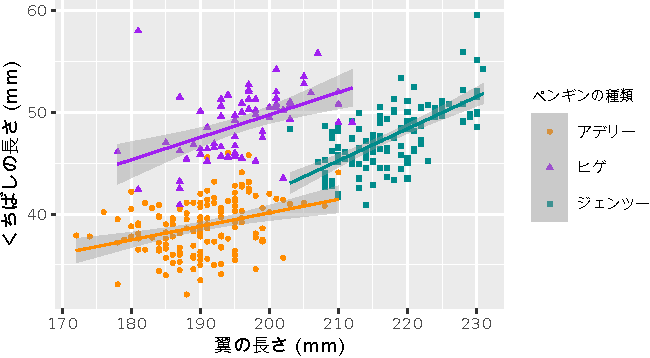
\includegraphics{kut_econ_thesis_files/figure-latex/scat1-1.pdf}
\caption{\label{fig:scat1}ペンギンの翼の長さとくちばしの長さの関係}
\end{figure}

\section{考察}\label{ux8003ux5bdf}

分析結果からどのようなことがわかったか(わからなかったか)議論する。先行研究の知見との比較し、新たに明らかになったことをはっきさせる。さらに、今後の課題について確認する。

最後に、参照・引用の方法を確認する。文献の引用・参照には、.bib ファイルに記録された citation key を利用する。自分が引用・参照する文献の citation key は、文献管理アプリで確認する。参考文献は \texttt{myrefs.bib}という名前の1つのファイルにまとめて保存し、卒論の Rmd ファイルと同じフォルダに設置する必要がある\footnote{他のファイル名にする場合や複数ファイルを読み込みたい場合は、\texttt{kut\_econ\_thesis\_lualatex.tex} で.bibを呼び出す1行を書き換える。}。

このテンプレートは武田史郎氏が作成した \texttt{jecon.bst} という文献スタイルファイルに依存しているので、このファイルを武田氏の\href{https://github.com/ShiroTakeda/jecon-bst/}{GitHubページ} から入手し、卒論のRmdファイルと同じフォルダに設置する\footnote{やり方が分かるなら \texttt{texmf-local} に設置してシステム全体で利用できるようにインストールしてもよいが、ここでは説明しない。}。基本的な注意はそのページに書いてあるとおりだが、特に注意すべきは以下の3点である。

\begin{enumerate}
\def\labelenumi{\arabic{enumi}.}
\tightlist
\item
  日本語の著者名を書くときも、欧文著者名と同様に姓と名の間にカンマを入れる
\end{enumerate}

\begin{itemize}
\tightlist
\item
  例:\texttt{author\ =\ \{浅野,\ 正彦\ and\ 矢内,\ 勇生\}}
\end{itemize}

\begin{enumerate}
\def\labelenumi{\arabic{enumi}.}
\setcounter{enumi}{1}
\tightlist
\item
  日本語文献には、\texttt{langid\ =\ \{japanese\}} という項目を追加する
\item
  日本語文献には、 \texttt{yomi} という項目を追加して、著者または編者の名前の読み方を記す。
\end{enumerate}

\begin{itemize}
\tightlist
\item
  外国語文献(アルファベット順)と日本語文献(あいうえお順)を分けてリストを作りたいときは、\texttt{yomi} をひらがなで記す。

  \begin{itemize}
  \tightlist
  \item
    例:\texttt{yomi\ =\ \{あさの,\ まさひこ\ and\ やない,\ ゆうき\}}
  \end{itemize}
\item
  外国語文献と日本語文献を混在させてアルファベット順に並べたいときは \texttt{yomi} をローマ字で記す(このテンプレートはこちらを採用している)。

  \begin{itemize}
  \tightlist
  \item
    例:\texttt{yomi\ =\ \{asano,\ masahiko\ and\ yanai,\ yuki\}}
  \end{itemize}
\end{itemize}

具体例として、このテンプレートと一緒に配布した\texttt{myrefs.bib}を参照されたい。

本文中で\texttt{nishiyama2019} というcitation key が付けられた文献を参照する際は、「\citet{nishiyama2019} は計量経済学の優れた教科書である」のように @ を付けて参照する。Citation key の直後に半角スペースが必要なので注意されたい。文の最後のカッコ内に参照文献を示すときは、{[} {]} を使って、「統計的に有意な結果が実質的にも有意とは限らない \citep[たとえば、][pp.~165-168]{mayy2018}」のようにする。複数文献の参照はセミコロン\texttt{;} で区切り 、「統計的因果推論は難しい \citep{ang2015, cunningham2021}」とする。

\section{結論(or おわりに)}\label{ux7d50ux8ad6or-ux304aux308fux308aux306b}

最後に、論文で明らかになった知見をまとめて結論を述べる。「結びにかえて」などという節で終えずに、必ず結ぶこと。

R Markdown は便利である。R Markdown を使えば、プロジェクト研究のデータ分析と論文執筆をまとめて実行することができる。図表の貼り間違いや、数値の転記ミスなどの心配がなくなり、議論の中身に集中することができる。プロジェクト研究でデータ分析を行う学生は、このテンプレートを使って卒業論文を書くべきである。

Rでデータ分析を行うなら、このテンプレートを使わない理由がどこにあるのだろうか。

あいうえお \citet{moe1984}

\bibliographystyle{jecon}
\bibliography{myrefs}

\end{document}
